\documentclass[tikz,border=8pt]{standalone}
% Shared look for every TikZ diagram. Load with \input{../../tools/tikz-style.tex}
\usepackage[T1]{fontenc}
\usepackage{lmodern}
\renewcommand{\sfdefault}{lmr}  % diagrams use the same serif as the text
\usetikzlibrary{arrows.meta, positioning, shapes.geometric, calc, fit, backgrounds}
\definecolor{cblue}{HTML}{4C78A8}
\definecolor{corange}{HTML}{F58518}
\definecolor{cgreen}{HTML}{54A24B}
\definecolor{cred}{HTML}{E45756}
\definecolor{cpurple}{HTML}{B279A2}
\definecolor{cgrey}{HTML}{6B6B6B}
\tikzset{
  every picture/.style={font=\sffamily, line width=1.2pt},
  box/.style={draw=#1, fill=#1!12, rounded corners=4pt, align=center, inner sep=7pt, minimum height=1.1cm},
  box/.default=cgrey,
  arrow/.style={-{Stealth[length=3mm]}, draw=cgrey, line width=1.4pt},
  title/.style={font=\sffamily\bfseries\Large},
  note/.style={font=\sffamily\small, text=cgrey, align=center},
}
\AtBeginDocument{\hyphenpenalty=10000 \exhyphenpenalty=10000}

\begin{document}
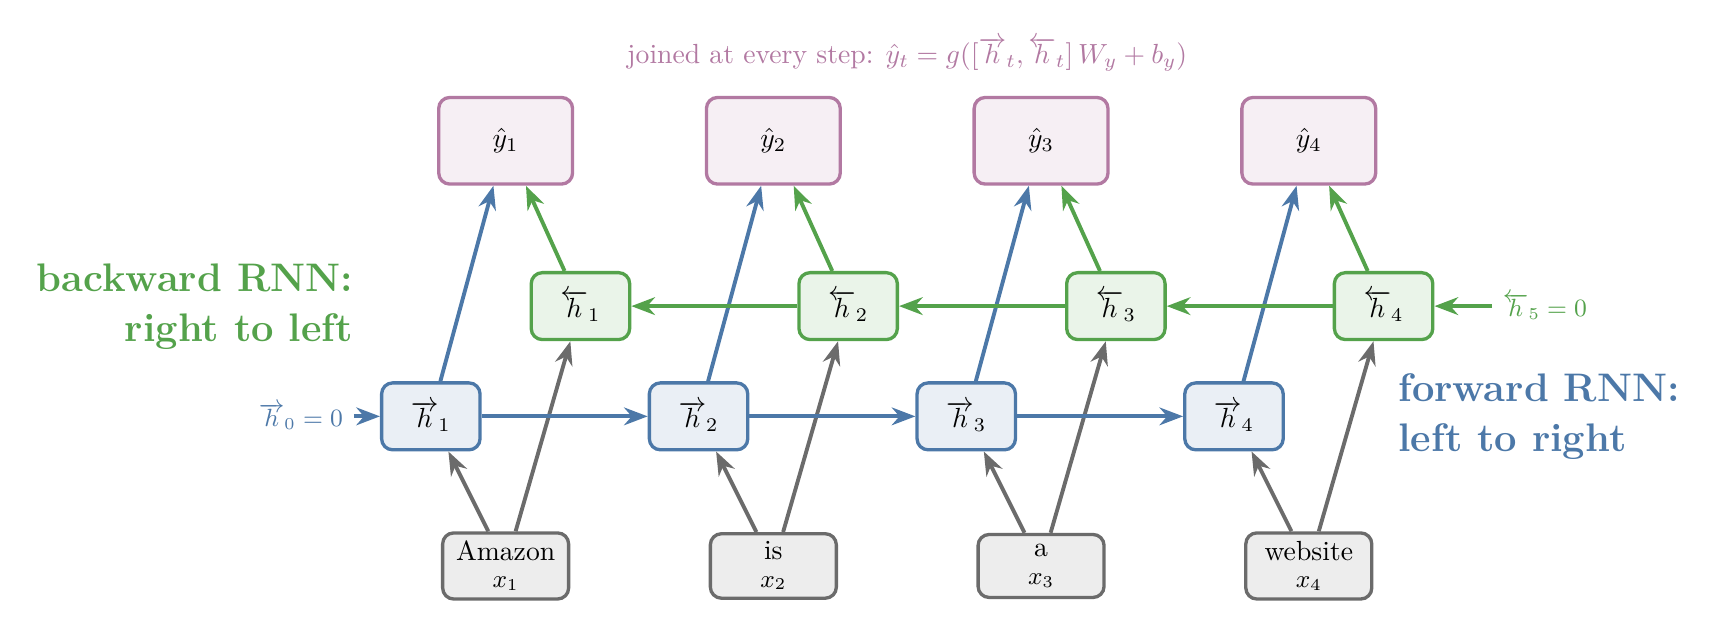
\begin{tikzpicture}[st/.style={box=#1, minimum width=1.25cm, minimum height=0.85cm, inner sep=2pt}]
  \foreach \t/\w in {1/Amazon,2/is,3/a,4/website} {
    \node[box=cgrey, minimum width=1.6cm, minimum height=0.8cm, inner sep=3pt] (x\t) at (3.4*\t,0) {\w\\[-2pt]{\small $x_\t$}};
    \node[st=cblue] (f\t) at (3.4*\t-0.95,1.9) {$\overrightarrow{h}_\t$};
    \node[st=cgreen] (b\t) at (3.4*\t+0.95,3.3) {$\overleftarrow{h}_\t$};
    \node[box=cpurple, minimum width=1.7cm, inner sep=3pt] (y\t) at (3.4*\t,5.4) {$\hat{y}_\t$};
    \draw[arrow, draw=cgrey] (x\t) -- (f\t);
    \draw[arrow, draw=cgrey] (x\t) -- (b\t);
    \draw[arrow, draw=cblue] (f\t) -- (y\t);
    \draw[arrow, draw=cgreen] (b\t) -- (y\t);
  }
  \foreach \a/\b in {1/2,2/3,3/4} {
    \draw[arrow, draw=cblue] (f\a) -- (f\b);
    \draw[arrow, draw=cgreen] (b\b) -- (b\a);
  }
  \node[note, text=cblue] (f0) at (0.8,1.9) {$\overrightarrow{h}_0 = 0$};
  \draw[arrow, draw=cblue] (f0) -- (f1);
  \node[note, text=cgreen] (b5) at (16.6,3.3) {$\overleftarrow{h}_5 = 0$};
  \draw[arrow, draw=cgreen] (b5) -- (b4);
  \node[title, text=cblue, anchor=west, align=left] at (14.6,1.9) {forward RNN:\\left to right};
  \node[title, text=cgreen, anchor=east, align=right] at (1.6,3.3) {backward RNN:\\right to left};
  \node[text=cpurple] at (8.5,6.5) {joined at every step: $\hat{y}_t = g([\overrightarrow{h}_t, \overleftarrow{h}_t]\, W_y + b_y)$};
\end{tikzpicture}
\end{document}
